\documentclass[]{article}

\usepackage[utf8]{inputenc}
\usepackage[paperheight=1.0in,paperwidth=2.1in,margin=0in]{geometry}
\usepackage{tikz}
\usetikzlibrary{shapes,arrows,automata,calc}
\usepackage{color}

\usepackage{booktabs}  % nicer table borders 

\begin{document}

%\clearpage
%\thispagestyle{empty}

\tiny{
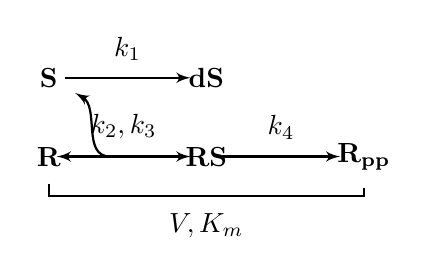
\begin{tikzpicture}[auto, outer sep=3pt, node distance=0cm,>=latex']

\node  at (-8.1, 8) (S) {$\bf S$};
\node  at (-6.1, 8) (dS) {$\bf dS$};
\draw [->, thick] ($(S)+(0.2,0)$) to node {$k_1$} ($(dS)+(-0.2,0)$);

\node  at (-8.1, 7) (R) {$\bf R$};
\node  at (-6.1, 7) (RS) {$\bf RS$};
\node  at ($(R)!0.5!(RS)$) (RRS) {};
\draw [<->, thick] ($(R)+(+.1,0)$) to node {$k_2, k_3$} ($(RS)+(-0.2, 0)$);
\draw [<-, thick] (S) edge[in=180, out=330] (RRS);
%\node  at (-3.8, 7.8) (X3) {$k_4^{cat},K_4m$};

\node at (-4.1, 7) (Rpp) {$\bf R_{pp}$};
\draw [->, thick] ($(RS)+(+.2,0)$) to node {$k_4$} ($(Rpp)+(-0.3, 0)$);
\node at (-4.1, 6.5) (downRpp) {};
\node at (-8.1, 6.5) (downR) {};
    \draw [-, thick] (Rpp) -- ($(downRpp)+(0,-.014)$);
    \draw [-, thick] (R) -- ($(downR)+(0,-.014)$);
    \draw [-, thick] (downRpp.center) to node {$V, K_m$} (downR.center);



\end{tikzpicture} 
}

\end{document}

